%
% This is the LaTeX template file for lecture notes for EE 382C/EE 361C.
%
% To familiarize yourself with this template, the body contains
% some examples of its use.  Look them over.  Then you can
% run LaTeX on this file.  After you have LaTeXed this file then
% you can look over the result either by printing it out with
% dvips or using xdvi.
%
% This template is based on the template for Prof. Sinclair's CS 270.

\documentclass[twoside]{article}
\usepackage{graphics}
\setlength{\oddsidemargin}{0.25 in}
\setlength{\evensidemargin}{-0.25 in}
\setlength{\topmargin}{-0.6 in}
\setlength{\textwidth}{6.5 in}
\setlength{\textheight}{8.5 in}
\setlength{\headsep}{0.75 in}
\setlength{\parindent}{0 in}
\setlength{\parskip}{0.1 in}
\usepackage{graphicx}


%
% The following commands set up the lecnum (lecture number)
% counter and make various numbering schemes work relative
% to the lecture number.
%
\newcounter{lecnum}
\renewcommand{\thepage}{\thelecnum-\arabic{page}}
\renewcommand{\thesection}{\thelecnum.\arabic{section}}
\renewcommand{\theequation}{\thelecnum.\arabic{equation}}
\renewcommand{\thefigure}{\thelecnum.\arabic{figure}}
\renewcommand{\thetable}{\thelecnum.\arabic{table}}

%
% The following macro is used to generate the header.
%
\newcommand{\lecture}[4]{
   \pagestyle{myheadings}
   \thispagestyle{plain}
   \newpage
   \setcounter{lecnum}{#1}
   \setcounter{page}{1}
   \noindent
   \begin{center}
   \framebox{
      \vbox{\vspace{2mm}
    \hbox to 6.28in { {\bf EE 382N: Distributed Systems
                        \hfill Fall 2017} }
       \vspace{4mm}
       \hbox to 6.28in { {\Large \hfill Lecture #1: #2  \hfill} }
       \vspace{2mm}
       \hbox to 6.28in { {\it Lecturer: #3 \hfill Scribe: #4} }
      \vspace{2mm}}
   }
   \end{center}
   \markboth{Lecture #1: #2}{Lecture #1: #2}
   %{\bf Disclaimer}: {\it These notes have not been subjected to the
   %usual scrutiny reserved for formal publications.  They may be distributed
   %outside this class only with the permission of the Instructor.}
   \vspace*{4mm}
}

%
% Convention for citations is authors' initials followed by the year.
% For example, to cite a paper by Leighton and Maggs you would type
% \cite{LM89}, and to cite a paper by Strassen you would type \cite{S69}.
% (To avoid bibliography problems, for now we redefine the \cite command.)
% Also commands that create a suitable format for the reference list.
\renewcommand{\cite}[1]{[#1]}
\def\beginrefs{\begin{list}%
        {[\arabic{equation}]}{\usecounter{equation}
         \setlength{\leftmargin}{2.0truecm}\setlength{\labelsep}{0.4truecm}%
         \setlength{\labelwidth}{1.6truecm}}}
\def\endrefs{\end{list}}
\def\bibentry#1{\item[\hbox{[#1]}]}

%Use this command for a figure; it puts a figure in wherever you want it.
%usage: \fig{NUMBER}{SPACE-IN-INCHES}{CAPTION}
\newcommand{\fig}[3]{
			\vspace{#2}
			\begin{center}
			Figure \thelecnum.#1:~#3
			\end{center}
	}
% Use these for theorems, lemmas, proofs, etc.
\newtheorem{theorem}{Theorem}[lecnum]
\newtheorem{lemma}[theorem]{Lemma}
\newtheorem{proposition}[theorem]{Proposition}
\newtheorem{claim}[theorem]{Claim}
\newtheorem{corollary}[theorem]{Corollary}
\newtheorem{definition}[theorem]{Definition}
\newenvironment{proof}{{\bf Proof:}}{\hfill\rule{2mm}{2mm}}

% **** IF YOU WANT TO DEFINE ADDITIONAL MACROS FOR YOURSELF, PUT THEM HERE:

\begin{document}
%FILL IN THE RIGHT INFO.
%\lecture{**LECTURE-NUMBER**}{**DATE**}{**LECTURER**}{**SCRIBE**}
\lecture{2}{August 18}{Vijay Garg}{Audrey Addison}
%\footnotetext{These notes are partially based on those of Nigel Mansell.}

% **** YOUR NOTES GO HERE:

% Some general latex examples and examples making use of the
% macros follow.  
%**** IN GENERAL, BE BRIEF. LONG SCRIBE NOTES, NO MATTER HOW WELL WRITTEN,
%**** ARE NEVER READ BY ANYBODY.
\section{Introduction}
This lecture covered material from Chapter 6, specifically, the User Datagram Protocol (UDP), the Transmission Control Protocol (TCP), and Java Remote Method Invocation (RMI).  

\textbf{Flash back - How to change the world?} \\
Thinking back to the early days of computing, the motivation for the lecture was: How do we connect 2 computers and change the world!?  To begin, we supposed we had two computers connected by wires.  

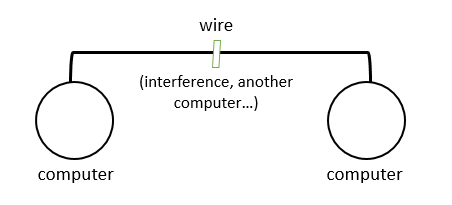
\includegraphics[scale=0.6]{img1.PNG}

\textbf{Key observations} \\
The physical world is not ideal. \\
We could have messages passing through another machine (congestion). \\
We may need to worry about the route the messages take. \\
Many things can go wrong. \\

\subsection{Layered software}
To help with this problem, the approach is to design your software in layers.  At the top, we have ``What I want", and the bottom, we have ``actual physical resources".  In between, we have many layers.  We start from the bottom with ``actual physical resources" and then incrementally improve the interface (reaching greater abstraction) as we progress through the layers from bottom to top until we reach the ``what I want". 

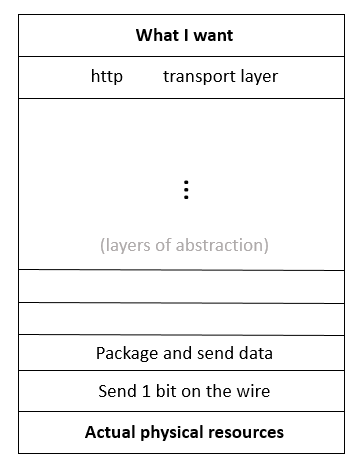
\includegraphics[scale=0.6]{img2.PNG}

For example, we may begin by sending 1 bit on the wire (that is a layer).  Then in the next layer, we may send one link or a group of bytes, and so on.

This approach is modular.  Individual layers can be swapped (provided the interfaces at the edges are consistent).  This is useful if you have multiple ways of doing the same thing. 


\section{Communicating with a server}

Flash back to modern day.  Now we have a distributed system and want to send a message.

Q: Who does this message go to?

A: We can specify this with the IP address of the machine (which could have multiple users) and the Port \#.
\\ \\
Q: How do we actually communicate?

A: By using either TCP or UDP protocols.

\subsection{User Datagram Protocol (UDP)}

Think of this like the US Postal Service.  You send a message by putting it in a package (envelope), giving it a TO address (IP address and port #) and a FROM address so the receiving server knows where the message came from.

Data is sent as ``\textbf{Datagram packets}".

This method is considered ``\textbf{not reliable}" in that one doesn't know if the message has been received.

But, it is \textbf{fast}.  It is \textbf{scalable} (no need to keep `per session' state).  Could handle millions of users.

How it works: there is a computer listening on a port (and some device to pick out ``bad packets") and anyone can send a packet.  As you send messages, they may arrive in order but - depending on the route - some packets could arrive out of order.  UDP does not inherently preserve message order (\textbf{not FIFO}).


\subsection{Transmission Control Protocol (TCP)}

Think of this like the phone (\textbf{session oriented}) or a pipe.  It is ``\textbf{reliable}" (messages are acknowledged as they are received).  But, there is a need to keep state for the session creating \textbf{more overhead} than UDP (e.g., slower).

TCP will slow you down if you try to send too much stuff (when the buffer is full).  There are lots of parameters one can adjust.  TCP \textbf{is FIFO} (it does preserve message order).

\subsection{Other protocols}

There is a Reliable UDP as well as many other protocols built upon TCP and UDP.  Almost everything is written on top of one of these.


\section{Implementing Protocols in java}

\subsection{UDP Implementation}

\textbf{See Datagram Packet (java class).}

Two methods: \\
  - send()    \\
  - receive()  \\
  
To start, we'll implement an ``echo server" (whatever message the server receives, it sends it back to the client).

\textbf{See: DatagramClient.java} \\

client creates \\
 - two DatagramPackets (declared on line 8, defined on line 22, 24), one for sending data (need hostname and port \#), one for receiving \\
 - one DatagramSocket (a UDP socket, line 15) \\
 
We use two methods from the DatagramPacket: \\
 - send (non-blocking call, line 23) \\
 - receive (blocking call, line 25) \\

Receive is on the server side, it is a \textbf{blocking call} meaning it can get stuck, or ``hang", until it receives a packet.

Class asides: \\
 - One could define a non-blocking receive. \\
 - We see the send call is made on line 23 and receive on line 25.  In reality, many things could happen between these calls. \\

\textbf{See: DatagramServer.java} \\

The server doesn't have to know who the client is until something is received.  Lines 17-18 give you the return address info.

\subsection{TCP Implementation}

For TCP, there are two types of sockets: \\ 
- ServerSocket (created by server using IP address and port \#) \\
    - then make blocking call while you wait for a call (``accept") \\
- Socket (per session, established by the client)\\

Server will maintain a table (public class NameTable) \\
 - table contains process name, IP address and port \# \\
 - table is searchable and editable by the client (see line 11, 19, 31) \\

``synchronized" keyword because server is multithreaded. \\

``getSocket()" call \\
 - establishes connection with server \\
 - socket is TCP Socket \\
 - symbols --- server name and port (line 8) \\
 - get 1 input stream (read) \\
 - get 1 output stream (write) \\
   (think of these as an input pipe and an output pipe) \\

\section{RMI}

These methods work well, but the programmer does have to do a lot of work packing and unpacking strings, parsing them...  We would like to abstract away some of the message passing.

\textbf{Q: Can we do better?} \\
Why do we have to accept a string and then unpack and parse it?

\textbf{A: Remote Procedure Call (RPC), then... Remote Method Invocation (RMI)} \\
With these, the compiler does the ``marshalling" and ``unmarshalling" \\
We have the notion of a ``remote object" (e.g., the server table) with an interface (methods you can call) \\

\textbf{Code example:} \\
NameRMIClient:  (NameServiceImpl.java?)\\
Client side: \\
 - find the remote object (using the rmiregistry daemon which maintains list of registered objects) \\
 - line 7 - port \# is implicit \\
 - just want a handle to the object (r is a reference, the object lives on the server side) \\ \\
Also have to worry about security (line 22) \\

NameService: \\
 - need this interface on both client and server side to compile \\
 - throws Remote Exception \\
 
\subsection{Parameter passing} 

If you have a function that sends a reference to an object (from client side to server side or vice versa), you will have trouble.  That reference doesn't mean anything on the other machine. \\

\textbf{Calling the function:  foo(object p)} \\
2 solutions: \\
 1) serialize the object p (inefficient if p is large, complicated if p also contains references within itself) \\
 2) make p also remote \\
 
\textbf{Calling the function:  foo(int z)} \\
 - send primitive types by value \\
 
Overall, be careful with parameters. \\
 - send primitive types by value \\
 - if an object, it can be local or remote \\
 - send local objects by serialization - beware of overhead on large objects \\
 - send remote objects by proxy \\

\section{To do:}

Read the class notes. \\

Security Policy File (specified by user, outlines constraints for the security manager to enforse) \\
 - google Java RMI tutorial (Oracle) \\
 
Be aware there are many other types of protocols: http, web services... \\



\end{document}





